\chapter{背景知识及相关工作}
本文的研究重点是开源软件漏洞的补丁定位问题,本章将首先介绍漏洞相关的背景知识,包括:通用漏洞披露(CVE)、漏洞通告(advisory)和漏洞补丁(vulnerability patch);然后,从漏洞披露信息的质量、漏洞补丁的分析及应用三个方面介绍相关的研究工作。


\section{背景知识}
% 本小节主要介绍本文工作中的背景知识,包括:通用漏洞披露(CVE)、漏洞通告(advisory)和漏洞补丁(vulnerability patch)。

\subsection{CVE及NVD} 
% 重平台
% 是什么? 有哪些信息?举个例子? 
% 作为community的source,还有其他的third party db、sources?
% 有什么作用? 被哪些其他 official、third-party report引用
通用漏洞披露(Common Vulnerabilities and Exposures,CVE)\cite{mitre2021:cve},是一个与网络安全有关的漏洞字典,收集各种信息安全漏洞并给予唯一编号以便于公众查阅及引用\footnote{https://cve.mitre.org/cve/}。在实际使用中,当人们提及某个CVE时,他们其实是在说某个被分配了CVE-ID的安全漏洞\footnote{https://www.redhat.com/en/topics/security/what-is-cve}。
\begin{figure}[h]
    \centering
    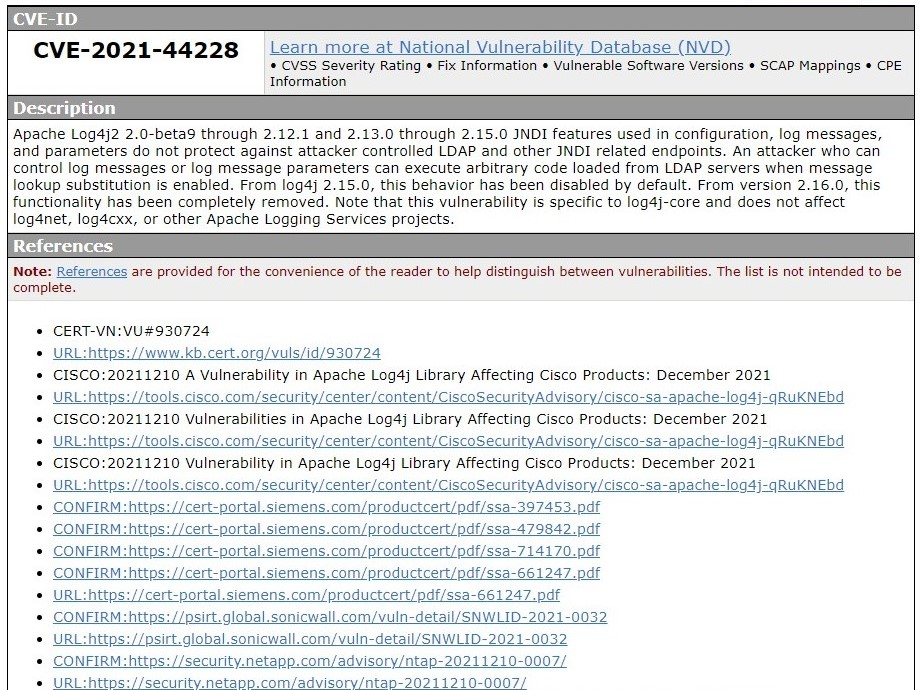
\includegraphics[width=0.88\textwidth]{res/CVE-2021-44228-2}
    \caption{CVE平台中漏洞CVE-2021-44228信息}
    \label{fig:CVE-2021-44228}
\end{figure}

每一个CVE条目(CVE Entry)都有唯一通用标识符(即:CVE-ID)、一段漏洞描述(即:Description)以及至少一个引用链接(即:References),该引用链接多为外部网站且包含与该漏洞相关的更详细的描述信息。如图例\ref{fig:CVE-2021-44228}所示为CVE-2021-44228\footnote{https://cve.mitre.org/cgi-bin/cvename.cgi?name=CVE-2021-44228},漏洞的描述信息为:“Apache Log4j2 2.0-beta9 through 2.12.1 and 2.13.0 through 2.15.0 JNDI features used in configuration, ...... Note that this vulnerability is specific to log4j-core and does not affect log4net, log4cxx, or other Apache Logging Services projects.”,且包含多个引用链接,如:“https://www.kb.cert.org/vuls/id/930724”等URL。

\begin{figure}[h]
    \centering
    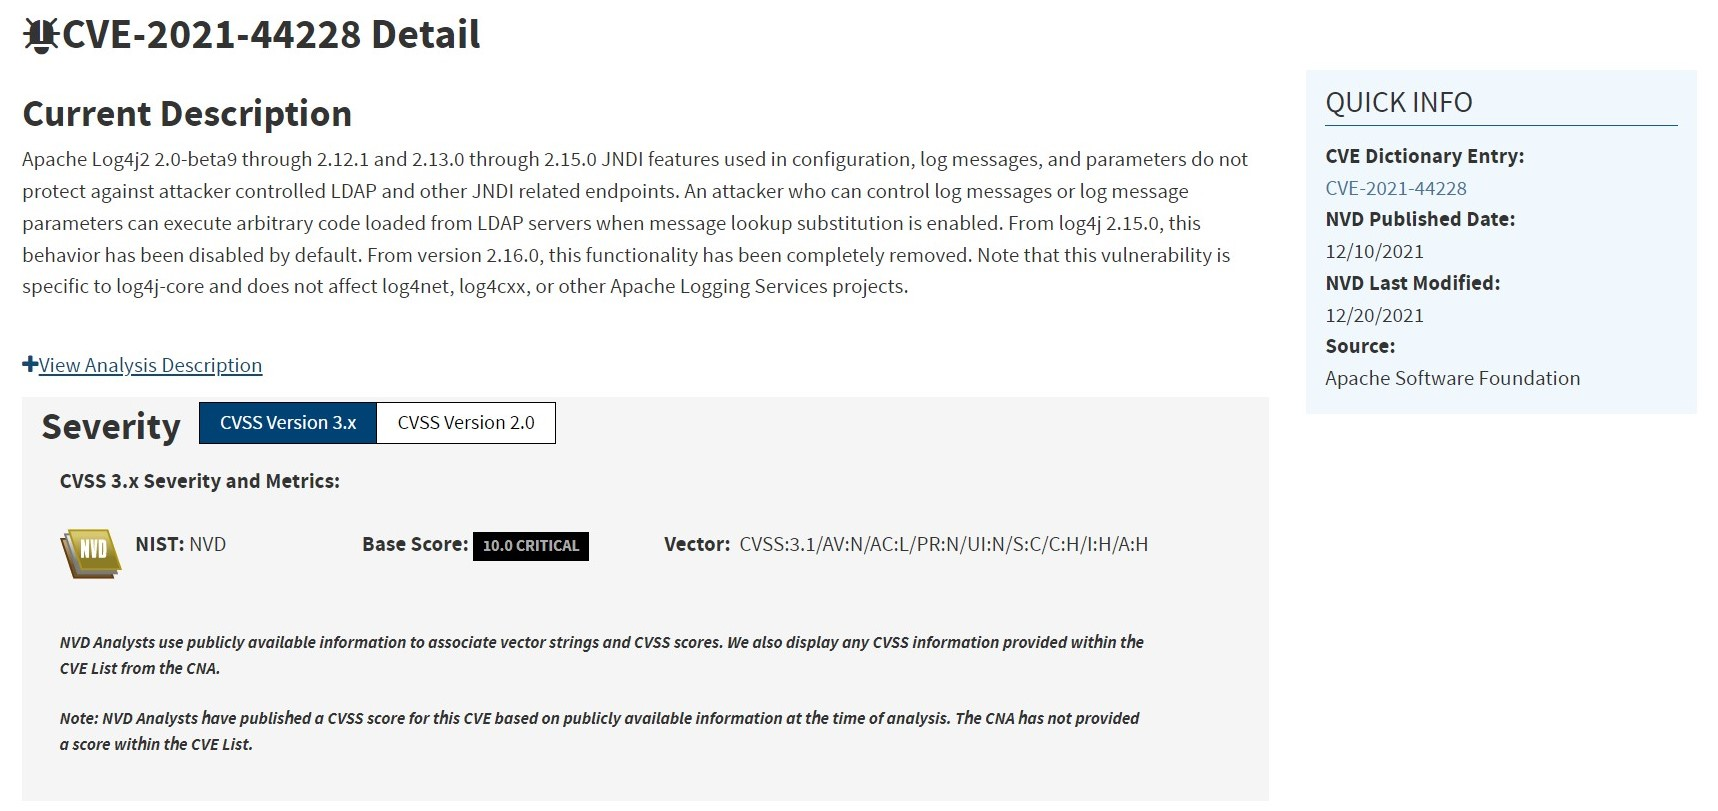
\includegraphics[width=1.0\textwidth]{res/NVD-2021-44228}
    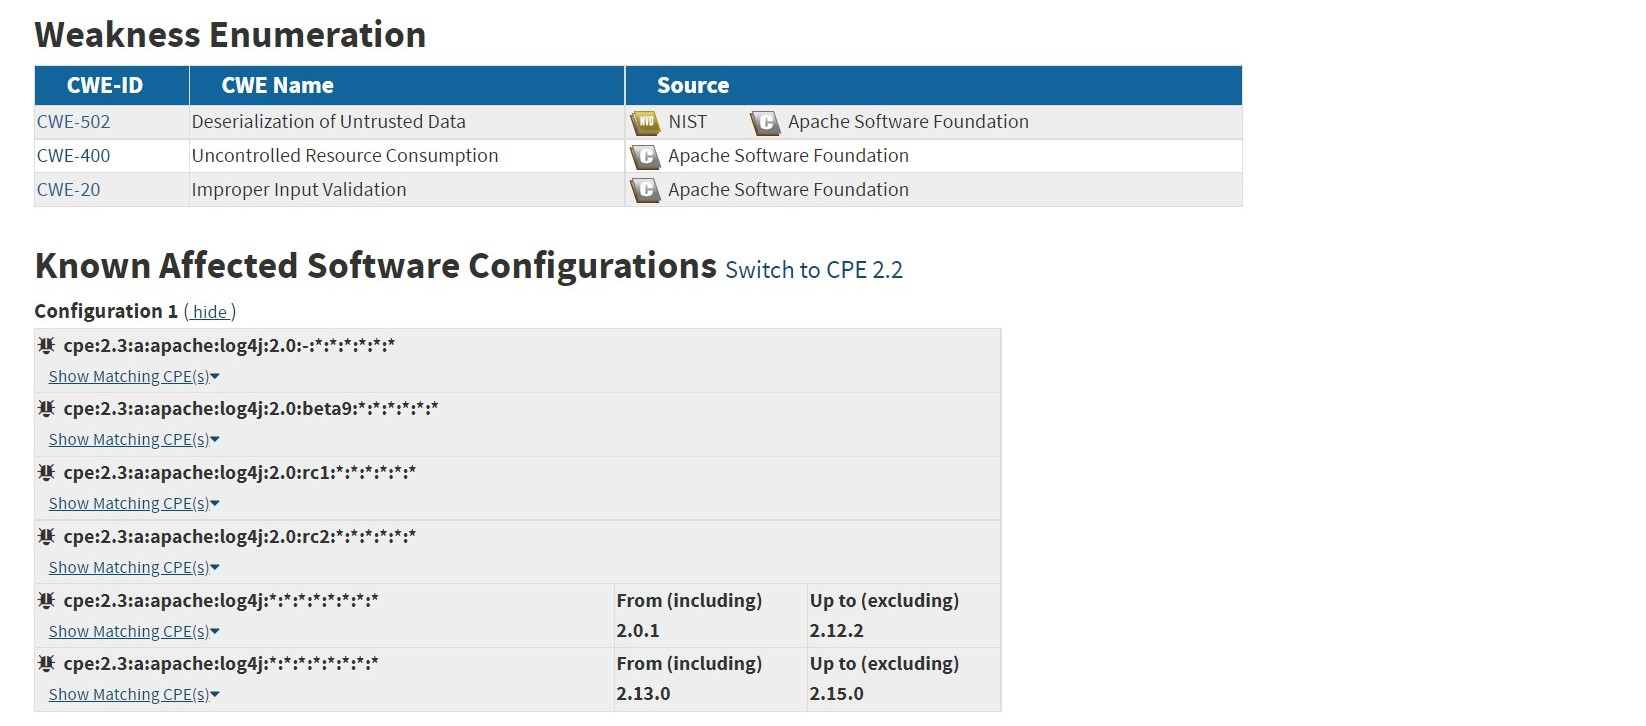
\includegraphics[width=1.0\textwidth]{res/NVD-2021-44228-2}
    \caption{NVD平台中漏洞CVE-2021-44228信息}
    \label{fig:NVD-2021-44228}
\end{figure}

CVE被设计作为漏洞字典用于收录并编号漏洞,这也导致CVE中漏洞信息过于精简,仅有一段漏洞描述和引用链接信息。基于CVE平台收录的漏洞条目信息,美国国家漏洞数据库(NVD)\footnote{https://nvd.nist.gov/}、中国国家信息安全漏洞库(CNNVD)\footnote{http://www.cnnvd.org.cn/}等漏洞数据库被构建,与CVE平台数据完全同步,并为每个漏洞条目(CVE Entry)提供更丰富的信息,如:影响的软件名及版本、修复信息、严重性评分、影响评级等。如图\ref{fig:NVD-2021-44228}所示为NVD平台中漏洞CVE-2021-44228\footnote{https://nvd.nist.gov/vuln/detail/CVE-2021-44228}信息。



\subsection{漏洞公告} 
% 是什么? 有哪些信息? 有哪些种(official、third-party)?举个例子?
漏洞公告(Advisory),也称漏洞通告,是由一般是由受漏洞影响的软件的厂商(Vendor)对外发布的安全漏洞警报,一般包含:漏洞触发描述、漏洞影响结果、漏洞软件名、软件版本等漏洞描述信息,有时也会包含漏洞发现者、漏洞修复记录、漏洞补丁等信息。

\begin{figure}[h]
    \centering
    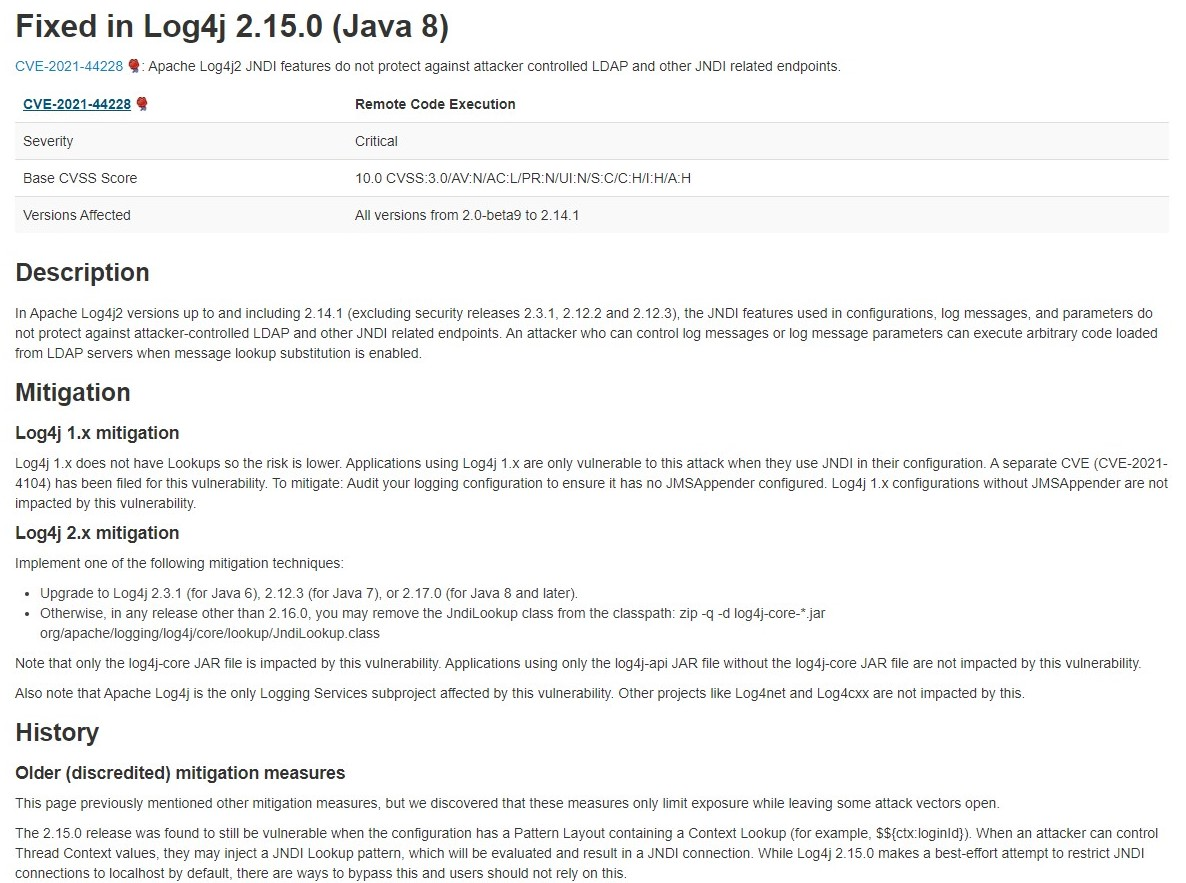
\includegraphics[width=0.88\textwidth]{res/Vendor-2021-44228}
    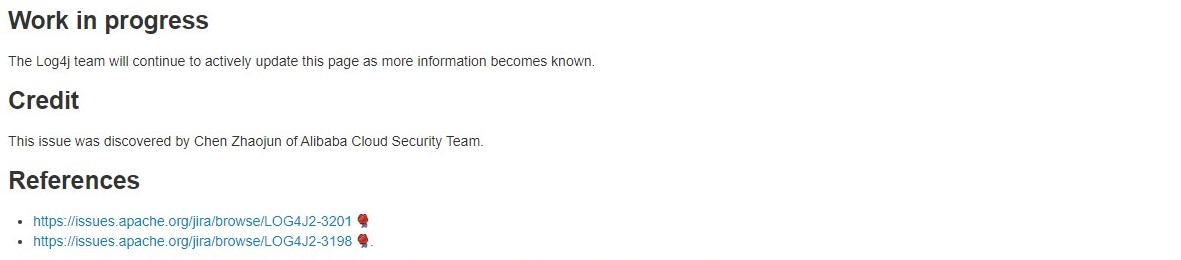
\includegraphics[width=0.88\textwidth]{res/Vendor-2021-44228-2}
    \caption{Apache Log4j发布的漏洞公告(CVE-2021-44228)}
    \label{fig:Vendor-2021-44228}
\end{figure}

如图\ref{fig:Vendor-2021-44228}所示为厂商Apache发布的关于CVE-2021-44228的漏洞公告\footnote{https://logging.apache.org/log4j/2.x/security.html},其中包含:修复方式“Log4j 2.x mitigation ...... Upgrade to Log4j 2.3.1 (for Java 6), 2.12.3 (for Java 7), or 2.17.0 (for Java 8 and later)”、漏洞发现者“Credit:This issue was discovered by Chen Zhaojun of Alibaba Cloud Security Team.”、引用链接“https://issues.apache.org/jira/browse/LOG4J2-3198”等信息。


以上由厂商发布的漏洞公告,也常被称为:厂商公告(Vendor Advisory);但由于某一厂商只会维护与该厂商相关的软件漏洞通告,开源社区的开发人员难以一一关注所有厂商的公告信息。因此,出现了许多第三方平台收集并维护所有漏洞公告信息,被称为:第三方公告(Third-party Advisory),例如:Red Hat\footnote{https://access.redhat.com/errata/}、Debian\footnote{https://www.debian.org/security/}、Gentoo\footnote{https://security.gentoo.org/}等。

% 官方或第三方?再顺路引出相关的sources,作为例子。

% Vender advisory, official advisory:CVE NVD,third-party advisory:Redhat debian 啥啥
% 是什么? 有哪些信息? 有哪些种(official、third-party:权威或非权威啥啥啥。。。社区、工业啥啥、、、)?举个例子?

\begin{figure}[h]
    \centering
    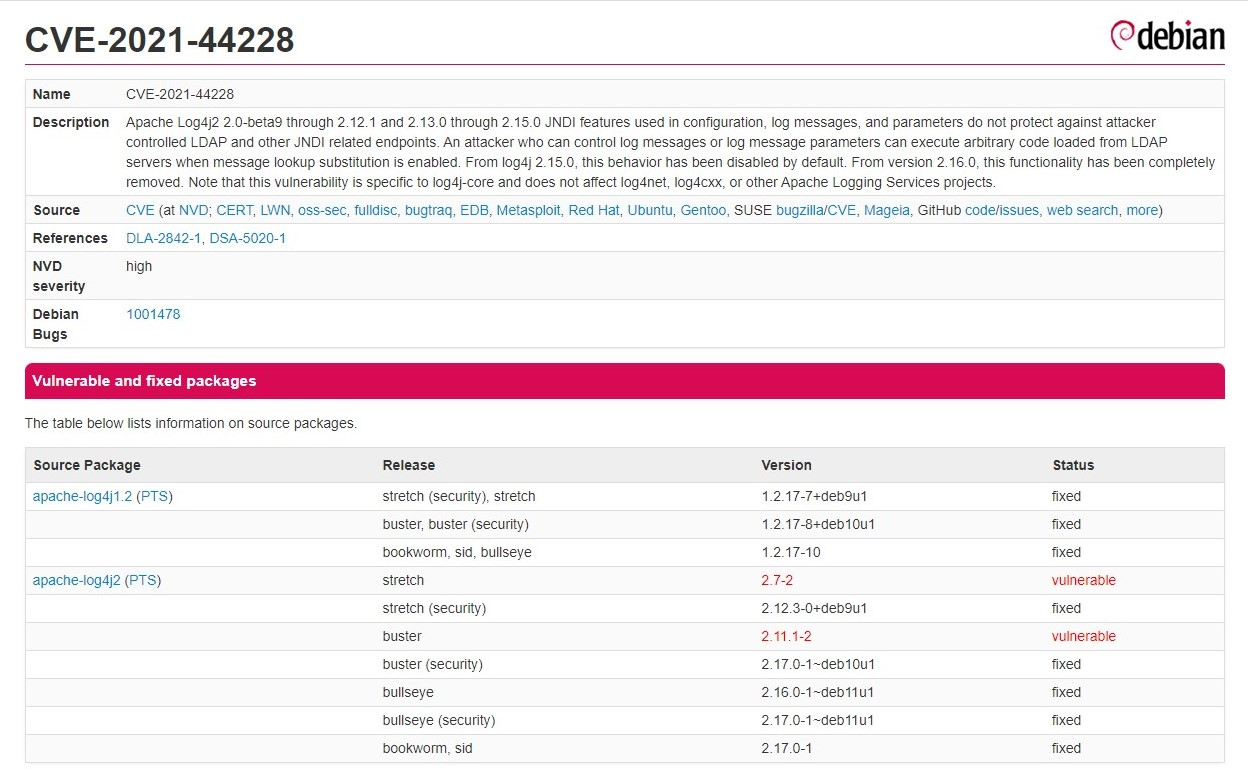
\includegraphics[width=0.88\textwidth]{res/debian-2021-44228}
    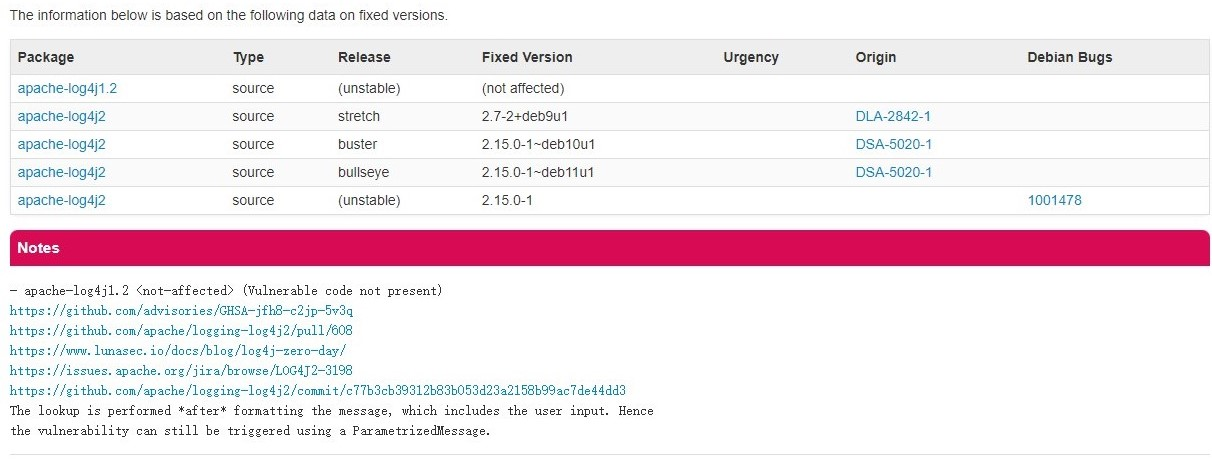
\includegraphics[width=0.88\textwidth]{res/debian-2021-44228-2}
    \caption{Debian平台中漏洞CVE-2021-44228信息}
    \label{fig:debian-2021-44228}
\end{figure}
如图\ref{fig:debian-2021-44228}所示为Debian平台中漏洞CVE-2021-44228信息\footnote{https://security-tracker.debian.org/tracker/CVE-2021-44228},其中还甚至包括了该漏洞的补丁提交信息\footnote{https://github.com/apache/logging-log4j2/commit/c77b3cb39312b83b053d23a2158b99ac7de44dd3}(图中“Note”中的URL引用链接),这在NVD以及Vendor Advisory中都未出现。


\subsection{漏洞补丁}
补丁(Patch),也称:补丁程序,是指对计算机程序进行的一组更改,旨在更新其功能或修复其缺陷。漏洞补丁(Vulnerability Patch)则指为修复程序中的安全漏洞所开发的补丁,通常以代码提交(Git和SVN Commit),或文本文件(.patch文件)等形式。

如图\ref{fig:debian-2021-44228}中的URL引用链接“https://github.com/apache/logging-log4j2/commit/\\c77b3cb39312b83b053d23a2158b99ac7de44dd3” (Github Commit),即为漏洞CVE-2021-44228的补丁,补丁内容见图\ref{fig:debian-2021-44228}。

\begin{figure}[h]
    \centering
    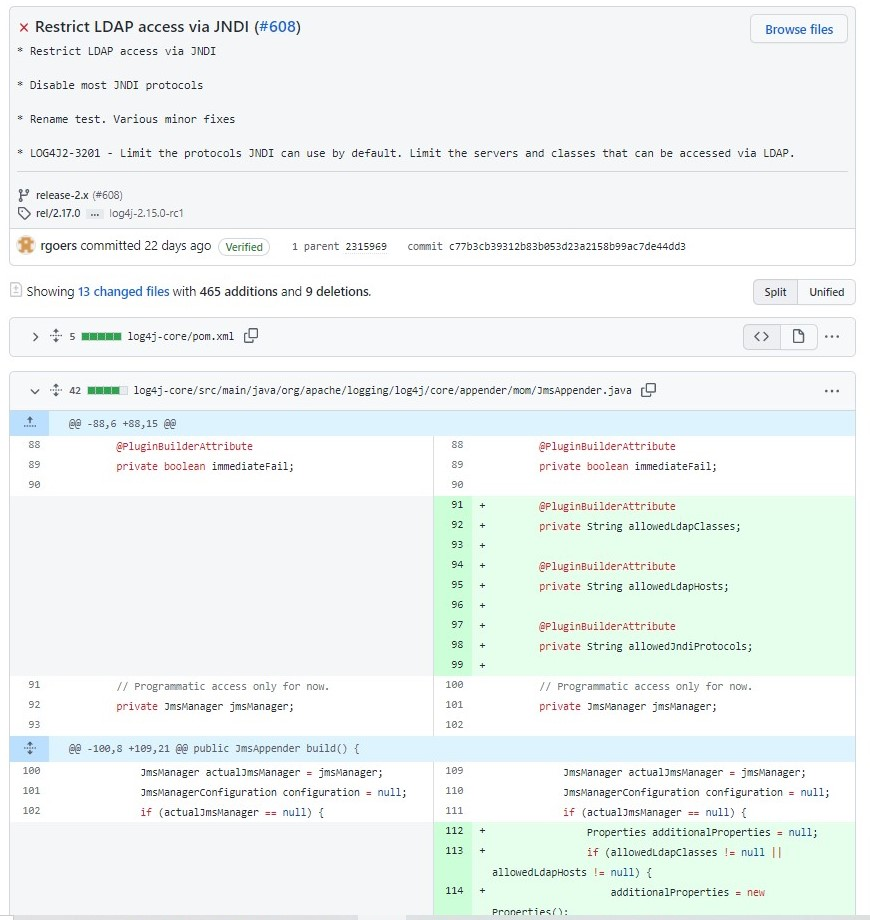
\includegraphics[width=0.88\textwidth]{res/commit-2021-44228}
    \caption{漏洞CVE-2021-44228的Github Commit补丁}
    \label{fig:commit-2021-44228}
\end{figure}



\section{相关工作}
\subsection{漏洞信息质量}
漏洞数据库(例如:CVE、NVD)被广泛关注,其中的漏洞信息也被广泛参考使用。随着漏洞数据库积累的漏洞数据越来越多,研究人员也越来越关注其中的漏洞信息的质量。

Nguyen和Massacci\cite{nguyen2013reliability}最早揭示了NVD数据库中漏洞所影响的软件版本信息的不可靠性。为了提高该信息的可靠性,Nguyen\cite{nguyen2016automatic}和Dashevskyi等人\cite{dashevskyi2018screening}开发了工具以确定某一旧软件版本是否会受到新披露的漏洞的影响。他们认为:如果旧版本包含修复漏洞所更改的源代码行,则该版本被视为受漏洞影响。Dong等人\cite{dong2019towards}从漏洞的描述信息中识别受漏洞影响的软件名称和版本,并与漏洞报告所提供的软件名称和版本信息进行对比。他们发现漏洞数据库中会遗漏真正受漏洞影响的版本,也会错误地包含了不受漏洞影响的版本。Chen等人\cite{chen2020automated}识别受漏洞影响的开源库信息。Chaparro等人的工作\cite{chaparro2017detecting}检测漏洞描述中是否缺少用于重现漏洞的关键步骤或预期效果信息。Mu等人的工作\cite{mu2018understanding}揭示了漏洞报告丢失重现漏洞信息的普遍性。以上工作已侧重于漏洞信息的多个方面,而本文的工作重点则是研究漏洞的补丁信息,并尝试自动化地从不同来源漏洞报告的综合信息中定位漏洞补丁。
% \tocheck{jo等人}\cite{jo2020gapfinder}识别网络安全领域内的语义不一致。
% \tocheck{这些工作侧重于漏洞信息的不同方面。按照这个方向,我们的工作重点是漏洞补丁,并尝试从漏洞报告的综合来源中识别漏洞补丁。}

近期,Tan等人完成了一项与本文的研究问题相似的工作\cite{Tan2021locating}。他们使用深度学习排名算法对代码仓库中的提交(commit)历史进行排名,把排在首位的提交当作为漏洞的补丁提交。他们的工作包含两个假设:(1)CVE中,受漏洞影响的软件的代码仓库已知;(2)漏洞与其补丁提交在数量上是一对一的映射关系。然而,事实上,受漏洞影响的软件的代码仓库并不已知,而需人工识别;此外,漏洞与其补丁提交在数量上存在一对多的关系(Sec.\ref{sec:cardinality})。


\subsection{漏洞补丁分析}
当前,有多中补丁分析相关的任务可用于提高软件安全性,如:补丁的生成和部署\cite{mulliner2013patchdroid,duan2019automating,xu2020automatic}、补丁的存在性测试\cite{zhang2018precise,jiang2020pdiff,dai2020bscout}以及秘密补丁识别\cite{xu2017spain,zhou2017automated,sabetta2018practical,chen2020machine}。

此外,研究人员也已为Java\cite{ponta2019manually}、C/C++\cite{fan2020ac}以及特定开源项目\cite{jimenez2018enabling}构建安全补丁数据集。基于这些数据集,研究人员已开展实证研究以表征漏洞及其补丁\cite{zaman2011security,li2017large,liu2020large,antal2020exploring}。在这些工作中,补丁信息多由人工识别\cite{xu2020automatic,jiang2020pdiff,dai2020bscout,xu2017spain,zhou2017automated,sabetta2018practical,chen2020machine,ponta2019manually,zaman2011security},或通过启发式规则识别,例如:在CVE的引用链接中查找补丁提交信息\cite{duan2019automating,fan2020ac,jimenez2018enabling,li2017large,liu2020large},以及在提交信息(commit message)中搜索CVE标识符\cite{fan2020ac, jimenez2018enabling, antal2020exploring}。这些工作存在的问题为:通过人工收集成本过高,且耗时较长;然而,启发式规则的方法又不足以找到或是找全补丁。


\subsection{漏洞补丁应用}
漏洞补丁信息可被用于多种软件安全性任务。例如,基于漏洞补丁生成漏洞攻击程序\cite{brumley2008automatic,you2017semfuzz},通过软件成分分析以确定项目是否使用包含漏洞的第三方库,并判定该漏洞所影响的函数是否被调用\cite{pashchenko2018vulnerable,ponta2020detection,pashchenko2020vuln4real,Wang2020empirical},以及通过学习漏洞特征\cite{li2016vulpecker,li2018vuldeepecker,zhou2019devign,jimenez2019importance}、通过匹配漏洞签名\cite{jang2012redebug,kim2017vuddy}、通过匹配漏洞和补丁检测签名\cite{xu2020patch,xiao2020mvp,cui2020vuldetector}来检测程序中的漏洞。


与上一小结的补丁分析工作类似,这些工作中的CVE补丁主要通过人工识别\cite{pashchenko2018vulnerable,ponta2020detection,pashchenko2020vuln4real,xiao2020mvp}、基于启发式规则的方法\cite{li2016vulpecker,li2018vuldeepecker,you2017semfuzz,Wang2020empirical,jimenez2019importance}或直接取自为特定项目建立CVE和补丁之间映射关系的安全公告\cite{jang2012redebug,kim2017vuddy,xu2020patch}。但是,人工识别的成本过高,而且基于启发式规则的方法找到或是找全补丁。